\chapter{引论}

\section{关于这门课程}
    
    \subsection{课程性质}

        原理性课程: 基础性, 科学性, 普适性; 针对性差

    \subsection{学习的目的}

        \begin{itemize}
            \item 实现(通用)编译器
            \item 实现专用编译器
            \item 学习编译思想 \\
                计算思维: 抽象, 自动化
        \end{itemize}

    \subsection{如何学}

        \begin{itemize}
            \item 把握三年级的特点
            \item 纪律: 准时到, 认真听, 注意记
            \item 注意学习方法
        \end{itemize}

\section{什么叫编译程序}

    \begin{description}
        \item[翻译程序]    把某一种语言程序(称为\textsf{源语言程序})等价地转换成另一种语言程序(称为\textsf{目标语言程序})的程序.

        \item[编译程序]    把某一种高级语言程序等价地转换成另一种低级语言程序(如汇编语言或机器语言程序)的程序. 高级语言源程序通过编译程序生成面向机器的代码, 可能需要用到汇编程序和装配程序.

            \begin{description}
                \item[诊断编译程序] 专门用于帮助程序开发和调试的编译程序
                \item[优化编译程序] 着重于提高目标代码效率的编译程序
                \item[交叉编译程序] 产生不同于其宿主机的机器代码
                \item[可变目标编译程序] 不需重写编译程序中与机器无关的部分就能改变目标机的编译程序
            \end{description}

        \item[解释程序]    把源语言写的源程序作为输入, 但不产生目标程序, 而是边解释边执行源程序本身. 编译程序的许多构造与实现技术同样适用于解释程序.
    \end{description}

    \subsection{编译程序历史}

        \begin{itemize}
            \item 编译程序是系统软件中资格最老的成员之一
            \item 发展十分迅速和成熟
            \item 已经形成一套系统化的理论和技术
        \end{itemize}

    \subsection{编译理论与其他课程关系}

        以自动机和形式语言为基础, 用到数据结构和离散数学知识, 以操作系统为控制对象.

    \subsection{编译理论的应用}

        编译理论与方法是计算机科学与技术中理论和实践相结合的最好典范. ACM 图灵奖, 授予在计算机技术领域作出突出贡献的科学家, 程序设计语言, 编译理论与方法约占$1\over 3$.

        编译理论的许多想法和技术可以用于一般软件的设计. 如有穷状态技术用于文本编辑程序, 情报检索和模式识别, 上下文无关文法和语法制导翻译用于建立多种文本处理程序, 代码优化技术用于程序校验和由非结构化到结构化的程序转换.

\section{编译过程概述}

    \subsection{编译过程的组成}

        源程序通过\textbf{词法分析}分解为单词和符号, 通过\textbf{语法分析}被识别为语法单位, 通过\textbf{中间代码生成}产生中间代码, 通过\textbf{代码优化}和\textbf{目标代码生成}产生目标代码.

    \subsection{词法分析(lexical analysis)}

        任务: 扫描和分解字符串, 识别\{定义符, 标识符, 分界符, 运算符, 常数\}

        依据: 构词规则.

        主要理论基础: 自动机理论.

        描述词法规则的有效工具是正规式和有限自动机.

    \subsection{语法分析(syntax analysis)}

        任务: 在词法分析基础上将单词符号串转化为语法单位, 并确定整个输入串是否构成语法上正确的程序.

        依据: 语法规则

        主要理论基础: 上下文无关文法

        词法分析是一种线性分析, 而语法分析是一种层次结构分析.

    \subsection{语义分析和中间代码生成(IR generation)}

        任务: 在语法范畴进行初步翻译, 翻译成等价的中间语言.

        \textbf{中间语言}(intermediate representation)被认为是一种形式化的语言, 其中的一种叫做四元式.

        依据: 语义规则

        主要理论基础: 属性文法

    \subsection{中间代码优化(IR optimization)}

        任务: 对代码(主要是中间代码)进行加工变换, 在\textbf{执行结果相同}的情况下产生\textbf{时间和空间上}更高效的中间代码.

        依据: 程序等价变换规则

        主要理论基础: 数据流方程

        虽然名为optimization, 一般的实现是improvement, 并非寻找最优解.

    \subsection{目标代码生成(code generation)}

        任务: 将中间代码变换为\textbf{特定机器}上的低级机器语言代码

        \begin{itemize}
            \item 内存单元分配
            \item 寄存器分配
            \item 指令集选择
        \end{itemize}

        目标代码形式: 绝对指令, 可重定位指令, 汇编指令

        依据: 硬件体系结构, 指令系统

\section{编译程序的结构}

    编译全程伴随\textbf{表格管理}和\textbf{出错处理}.

    \subsection{表格管理}

        编译的各个阶段都要维护(许多)表格并进行表格管理以登记源程序的各类信息和编译各阶段的进展状况. 技术基础是数据结构, 表格的分类, 结构和处理方法取决于语言和特定的机器以及优化措施.

        编译程序涉及到的表格有符号名表, 常数表, 标号表, 入口名表, 过程引用表, 循环表, 等价名表, 公用链表, 格式表, 中间代码表等.

    \subsection{出错处理}
        
        一个好的编译器应当具有的特点:
        \begin{description}
            \item[全] 最大限度发现错误
            \item[准] 准确指出错误的性质和发生地点
            \item[局部化] 将错误的影响控制在尽可能小的范围内
        \end{description}

        自动纠正错误的代价较大. 源程序中的错误包括
        \begin{description}
            \item[语法错误] 不符合语法规则的错误, 如单词拼写出错, 括号不匹配
            \item[语义错误] 不符合语义规则的错误, 如说明错误, 作用域错误, 类型不匹配
        \end{description}

    \subsection{遍}

        \textsf{遍}(pass): 对源程序或源程序的中间结果\textbf{从头到尾扫描一次}并\textbf{做有关的加工处理}, 生成新的中间结果或目标程序. 不是每种语言都可以用单遍编译程序实现. C和C++特意设计为适合单遍编译程序, Java必须使用多遍编译.

    \subsection{编译的前端和后端}

        \textsf{前端}(front-end): 由与源语言有关但与目标机无关的部分组成, src$\to$scanner$\to$parser$\to$IR

        \begin{itemize}
            \item 词法分析
            \item 语义分析
            \item 产生中间代码
        \end{itemize}

        \textsf{后端}(back-end): 编译程序中与目标机有关的部分, IR$\to$选择指令$\to$寄存器分配$\to$机器代码

        目标机可变(平台无关)需要良好的中间语言, 如Java的Bytecode.

\section{编译程序生成}

    \subsection{编译程序的构造工具}

        一种自动化的做法: ``只给(词法, 语法, 语义, \ldots)规则, 要求得到编译器'', 规则要公式化(正规化). 规则就是语言. 这货真的存在.

        现在大多采用高级语言, 但核心部分或采用机器语言或汇编语言.

    \subsection{T型图}

        用高级语言写高级语言编译器的工具.

        \begin{figure}[h]\centering
            %\begin{minipage}{0.5\linewidth} \centering
                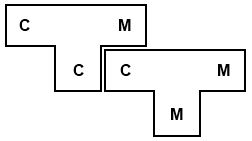
\includegraphics[width=5cm]{compile_chaps/lect2_inc/Bootstrapping-t-diagram.png}
                \caption{Bootstrapping-t-diagram}
                \label{fig:2:bootstrapping}
                % https://secure.wikimedia.org/wikipedia/en/wiki/File:Bootstrapping-t-diagram.png
                % 公有领域
            %\end{minipage}
        \end{figure}

        \begin{figure}[h] \centering
            \begin{minipage}{0.65\linewidth}
                \begin{center}
                {\small
\begin{verbatim}          +--------------+    +--------------+
          | L3        A0 |    | L3        A0 |
+---------+----+    +----+----+----+    +----+
| L2        A0 | L2 | L2        A0 | A0 |
+----+    +----+----+----+    +----+----+
     | L1 | L1        A0 | A0 |
     +----+----+    +----+----+
               | A0 |
               +----+\end{verbatim}}
                \end{center}
                \caption{3级自展技术(取自百度贴吧)}
                \label{fig:2:3-self-extract}
                % http://tieba.baidu.com/f?kz=387450349
            \end{minipage}
        \end{figure}


        可以用于软件移植.

    \subsection{自编译方式}

        思想: 先完成最核心的部分, 以它为工具构造一个能够编译更多语言成分的较大编译程序. 通过一系列自展途径而形成编译程序.

    \subsection{构造工具}

        编译程序产生器.

        已经完成的自动产生扫描器有lex, flex等, 自动产生语法分析器有yacc, Bison等

